\section{Results}


\subsection{Addressing Experimental Error}

Throughout all of the experiments, it was noted that there was a high amount of noise and variability in the results. Furthermore, taking measurements was difficult, as the voltage on the electrometer dropped from the moment the sample was placed in the ice pail. It was reasoned that this was due to a fault in the equipment. Possible reasons for this variability could be a grounding issue with the ice pail, a lack of electric insulation of the proof plane, a buildup of static charge on the person performing the experiment, or due to other external factors such as humidity.

Regardless of the source of error, five trials were performed to account for the randomness in results. It was ensured that each trial was entirely independent of the other to address any variables that may carry over. To achieve this, the proof plane was grounded between trials; in addition, the pail and shield of the ice pail were connected to discharge any residual charge still contained in the ice pail from previous experiments. Finally, the sampling sphere (in experiment 1) was set aside from the charged sphere before being grounded to not give the sampling sphere a net charge (this is further elaborated in the discussion for the first experiment).

\subsection{Error Analysis Methods}

Mathematical functions able to model the factors affecting charge distribution were beyond the scope of this experiment. Because of this, more analysis was done on the raw data and its relation to the expected theoretical value. Five trials are insufficient to calculate a standard deviation. Therefore, a maximum residual and maximum error was calculated for each point over multiple trials.

Mean:
$$  \overline{x} =\frac{\sum_{i=1}^{N} x_i  }{N}$$

Maximum Absolute Residual: 
$$\mathrm{MR}=\max \left(\left|x_i -\overline{x} \right|\right)$$

Maximum Error: 
$$\mathrm{ME}=\frac{\mathrm{MR}}{\sqrt{N}}$$


An additional residual calculation was performed in cases with a uniform charge density. This residual was calculated for every point with respect to the average charge of the entire sampling sphere. This "per-trial" residual gave an overall maximum residual comparing the charge at different points in a given trial. This residual calculation was done in conjunction with the established residual calculation that gave an overall maximum residual comparing the charge at the same points across the five trials.

Additionally, the digital display of the voltmeter (Model ES-9078A Electrometer) had an inherent uncertainty of $\pm$ 0.1V. While this does not take into account the experimental difficulties encountered with this instrument as discussed earlier, this was deemed a sufficient value of uncertainty. 

\newpage

\subsection{Experiment 1 - 2 spheres}

\begin{figure}[h]
    \centering
    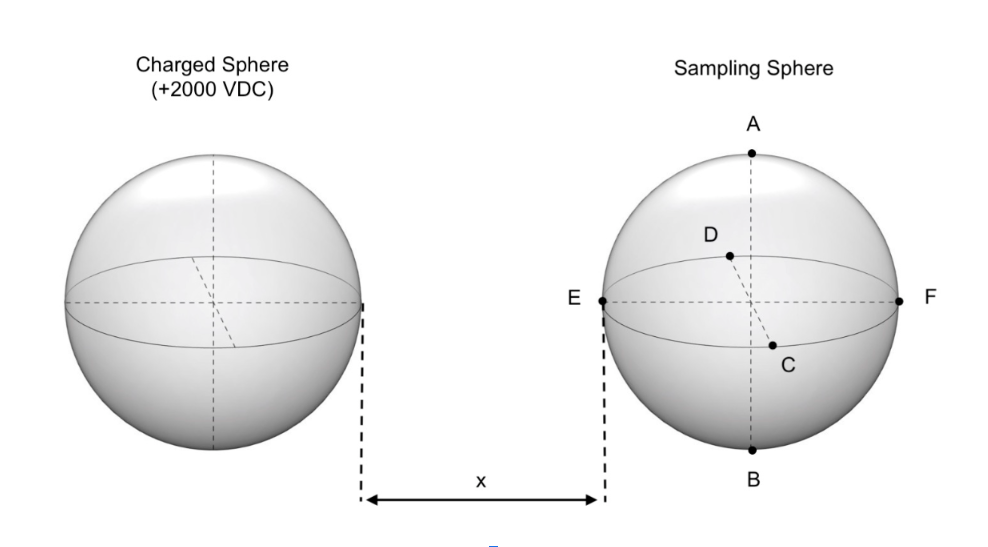
\includegraphics[height=5cm]{photos/experiment1image.png} % Adjust the height as needed
    \caption{Experiment 1: Model of the two conductive spheres, including the points measured}
    \label{fig:experiment1}
\end{figure}

\subsubsection{Part 1}

\begin{table}[h]
    \caption{\label{tab:table1}Results From Two Conductive Spheres 50 cm apart}
    \centering
    \begin{tabular}{@{}rllllllll@{}}
    \toprule
    & \multicolumn{8}{c}{\textbf{CHARGE (V)}}\\ \midrule
    \textbf{POINTS} &
      Trial 1 &
      \multicolumn{1}{c}{Trial 2} &
      \multicolumn{1}{c}{Trial 3} &
      \multicolumn{1}{c}{Trial 4} &
      \multicolumn{1}{c}{Trial 5} &
      \multicolumn{1}{c}{\textbf{Average}} &
      \multicolumn{1}{c}{\textbf{MR}} &
      \multicolumn{1}{c}{\textbf{ME}} \\
    A (Top)                  & 0.9  & 0.2  & 0    & 0   & -0.1 & 0.2  & 0.7  & 0.313049517                     \\
    B (Bottom)               & -0.4 & -0.1 & -0.1 & 0.1 & 0    & -0.1 & 0.3  & 0.134164079                     \\
    C (Front)                & 0.9  & 0.3  & 0    & 0.4 & 0.1  & 0.34 & 0.56 & 0.250439613                     \\
    D (Back)                 & 0.4  & 0.4  & 0.4  & 0.4 & 0.1  & 0.34 & 0.24 & 0.107331263                     \\
    E (Left)                 & 0.1  & 0.1  & 0    & 0.1 & 0.1  & 0.08 & 0.08 & 0.035777088                     \\
    F (Right)                & 0.8  & 0.9  & 0.3  & 0.3 & 0.1  & 0.48 & 0.42 & 0.18782971                      \\
    \textbf{Overall Average} & \multicolumn{8}{c}{0.223333333}                                                 \\
    \textbf{Overall MR}      & \multicolumn{8}{c}{0.676666667}                                                 \\
    \textbf{Overall ME}      & \multicolumn{8}{c}{0.123542}                                                    \\ \bottomrule
    \end{tabular}
\end{table}
    
The results from two conductive spheres 50 cm apart, as seen in Table~\ref{tab:table1}, show an extremely low voltage with an overall average of 0.22V. The different points on the sphere are similarly charged with very little difference between points. Therefore, the charges on the sphere can be considered uniform.

\newpage

\subsubsection{Part 2}

\begin{table}[h]
    \caption{\label{tab:table2}Results From Two Conductive Spheres 1 cm apart}
    \centering
    \begin{tabular}{@{}rllllllll@{}}
    \toprule
    & \multicolumn{8}{c}{\textbf{CHARGE (V)}} \\
    \midrule
    \textbf{POINTS} & Trial 1 & Trial 2 & Trial 3 & Trial 4 & Trial 5 & \textbf{Average} & \textbf{MR} & \textbf{ME} \\
    A (Top) & 0.4 & 0.5 & 0.6 & 0.3 & 0.4 & 0.44 & 0.16 & 0.071554175 \\
    B (Bottom) & -0.1 & -0.7 & -1.2 & -1.5 & -1.5 & -1 & 0.9 & 0.402492236 \\
    C (Front) & 0.4 & 0.3 & 0.3 & 0.3 & 0.1 & 0.28 & 0.18 & 0.080498447 \\
    D (Back) & 0.1 & 0.1 & -0.1 & -0.1 & 0.1 & 0.02 & 0.12 & 0.053665631 \\
    E (Left) & -6.3 & -6.2 & -7.1 & -5.3 & -6.5 & -6.28 & 0.98 & 0.438269324 \\
    F (Right) & 0.7 & 0.9 & 0.9 & 0.6 & 0.7 & 0.76 & 0.16 & 0.071554175 \\
    \bottomrule
    \end{tabular}
\end{table}

The results from two conductive spheres 1 cm apart, as seen in Table~\ref{tab:table2}, show a significant disparity in charge between point E(Left) and the other points on the sphere. Points A, C and D all have a roughly neutral charge(0.44 V, 0.28 V, 0.02 V), while points B and E have a negative charge(-1 V, -6.28 V), and point F has a slightly positive charge(0.76 V).

\subsubsection{Part 3}

\begin{table}[h]
    \caption{\label{tab:table 3}: Results From Two Conductive Spheres 1 cm apart, after momentarily grounding the sampling sphere}
    \centering
    \begin{tabular}{@{}rllllllll@{}}
    \toprule
    \multicolumn{1}{l}{} & \multicolumn{8}{c}{\textbf{CHARGE (V)}}                       \\ \midrule
    \multicolumn{1}{c}{\textbf{POINTS}} &
      \multicolumn{1}{c}{Trial 1} &
      \multicolumn{1}{c}{Trial 2} &
      \multicolumn{1}{c}{Trial 3} &
      \multicolumn{1}{c}{Trial 4} &
      \multicolumn{1}{c}{Trial 5} &
      \multicolumn{1}{c}{\textbf{Average}} &
      \multicolumn{1}{c}{\textbf{MR}} &
      \multicolumn{1}{c}{\textbf{ME}} \\
    A (Top)              & -1.1 & -1.5 & -0.1 & -0.3 & -0.7 & -0.74 & 0.76 & 0.339882333 \\
    B (Bottom)           & -2.5 & -0.8 & -1.3 & -1.1 & -1.6 & -1.46 & 1.04 & 0.465102139 \\
    C (Front)            & -1.3 & -1.4 & -1.2 & -0.9 & -0.3 & -1.02 & 0.72 & 0.321993789 \\
    D (Back)             & -0.8 & -1.4 & -0.7 & -0.6 & -2.6 & -1.22 & 1.38 & 0.617154762 \\
    E (Left)             & -8   & -5.5 & -7.4 & -8.5 & -6.7 & -7.22 & 1.72 & 0.769207384 \\
    F (Right)            & -0.4 & 0.5  & 0.5  & 0.6  & 0.7  & 0.38  & 0.78 & 0.348826604 \\ \bottomrule
    \end{tabular}
\end{table}

The results from two conductive spheres 1 cm apart after momentarily grounding the sampling sphere, as seen in Table~\ref{tab:table3}, show a significant charge disparity between point E(Left) and the other points on the sphere. Point E is significantly more negative than other points, with an average of -7.22 V. Point F is the only positive point with an average of 0.78 V. Points A, B, C, and D are all roughly similarly changed (-.074 V, -1.46 V, -1.02 V, -1.22 V).

\subsubsection{Part 4}

\begin{table}[h]
    \caption{\label{tab:table 4}: Results From Two Conductive Spheres 50 cm apart, after having momentarily grounded the sampling sphere in the previous step}
    \begin{tabular}{@{}rllllllll@{}}
    \toprule
    \multicolumn{1}{l}{}                         & \multicolumn{8}{c}{\textbf{CHARGE (V)}}                       \\ \midrule
    \multicolumn{1}{c}{\textbf{POINTS}} &
      \multicolumn{1}{c}{Trial 1} &
      \multicolumn{1}{c}{Trial 2} &
      \multicolumn{1}{c}{Trial 3} &
      \multicolumn{1}{c}{Trial 4} &
      \multicolumn{1}{c}{Trial 5} &
      \multicolumn{1}{c}{\textbf{Average}} &
      \multicolumn{1}{c}{\textbf{Residual}} &
      \multicolumn{1}{c}{\textbf{ME}} \\
    A (Top)                                      & -1.2 & -1.8 & -1.5 & -0.8 & -1.8 & -1.42 & 0.62 & 0.277272429 \\
    B (Bottom)                                   & -1.9 & -1.7 & -2.5 & -2   & -2   & -2.02 & 0.48 & 0.214662526 \\
    C (Front)                                    & -1.3 & -1.5 & -1.8 & -1.2 & -1.7 & -1.5  & 0.3  & 0.134164079 \\
    D (Back)                                     & -0.5 & -1.5 & -2   & -1.8 & -1.3 & -1.42 & 0.92 & 0.411436508 \\
    E (Left)                                     & -1.5 & -1.6 & -1.8 & -1.5 & -1.5 & -1.58 & 0.22 & 0.098386991 \\
    F (Right)                                    & -0.9 & -1.6 & -1.7 & -1.3 & -2   & -1.5  & 0.6  & 0.268328157 \\
    \multicolumn{1}{l}{\textbf{Overall Average}} & \multicolumn{7}{l}{-1.573333333}                &             \\
    \multicolumn{1}{l}{\textbf{Overall MR}}      & \multicolumn{7}{l}{1.073333333}                 &             \\
    \multicolumn{1}{l}{\textbf{Overall ME}}      & \multicolumn{7}{l}{0.195963}                    &             \\ \bottomrule
    \end{tabular}
\end{table}
    
The results from two conductive spheres 50 cm apart that were momentarily grounded while next to the charged sphere, as seen in Table~\ref{tab:table4}, show a uniform charge distribution with a net negative charge. All points have a roughly equal charge with an overall average of  -1.57V.

\newpage

\subsection{Experiment 2 - Conical Shape}

\begin{figure}[h]
    \centering
    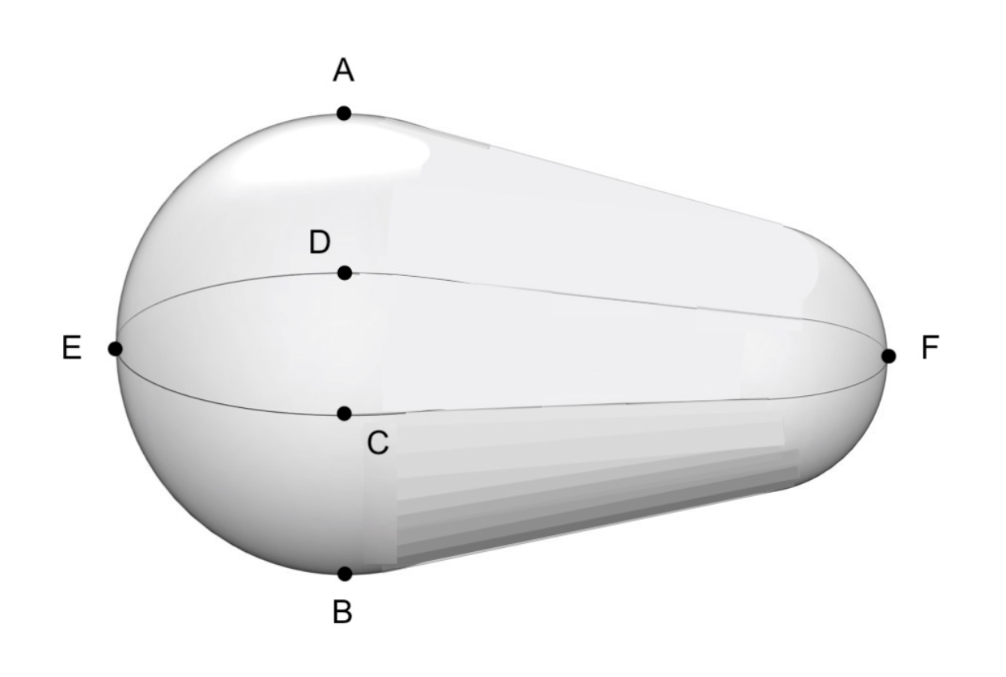
\includegraphics[height=5cm]{photos/experiment2image.png} % Adjust the height as needed
    \caption{Experiment 2: Conical Shape Diagram}
    \label{fig:experiment2}
\end{figure}

\begin{table}[h]
    \caption{\label{tab:table5}: Results From The Conductive Conical Shape}
    \begin{tabular}{@{}rllllllll@{}}
    \toprule
    \multicolumn{1}{l}{}   & \multicolumn{8}{c}{\textbf{CHARGE (V)}}                 \\ \midrule
    \multicolumn{1}{c}{\textbf{POINTS}} &
      \multicolumn{1}{c}{Trial 1} &
      \multicolumn{1}{c}{Trial 2} &
      \multicolumn{1}{c}{Trial 3} &
      \multicolumn{1}{c}{Trial 4} &
      \multicolumn{1}{c}{Trial 5} &
      \multicolumn{1}{c}{\textbf{Average}} &
      \multicolumn{1}{c}{\textbf{MR}} &
      \multicolumn{1}{c}{\textbf{ME}} \\
    A (Top)                & 5.2 & 4.9 & 5.9 & 5.7 & 6   & 5.54 & 0.64 & 0.286216701 \\
    B (Bottom)             & 4.8 & 5.4 & 4.9 & 4.7 & 4   & 4.76 & 0.76 & 0.339882333 \\
    C (Front)              & 6.9 & 5.6 & 4.6 & 5.3 & 4.9 & 5.46 & 1.44 & 0.643987578 \\
    D (Back)               & 6.4 & 4.8 & 5.2 & 5.8 & 5.3 & 5.5  & 0.9  & 0.402492236 \\
    E (Left -Larger end)  & 4.8 & 6   & 5.9 & 4.8 & 5.9 & 5.48 & 0.68 & 0.304105245 \\
    F (Right - Narrow end) & 8   & 7.8 & 7.6 & 6.6 & 7.2 & 7.44 & 0.84 & 0.37565942 \\ \bottomrule
    \end{tabular}
\end{table}
    
The results from the conductive conical shape, as seen in Table~\ref{tab:table5}, show a uniform charge on the larger end and a larger charge density on the narrower end. Points A, C, D and E have roughly similar charge densities (5.54 V, 5.46 V, 5.5 V, 5.48 V). Point B has a slightly lower charge density of 4.76 V. Point F( Right - Narrow end) has a higher charge density with an average of 7.44 V.
    
\newpage

\subsection{Experiment 3 - Hollow Sphere}

\begin{figure}[h]
    \centering
    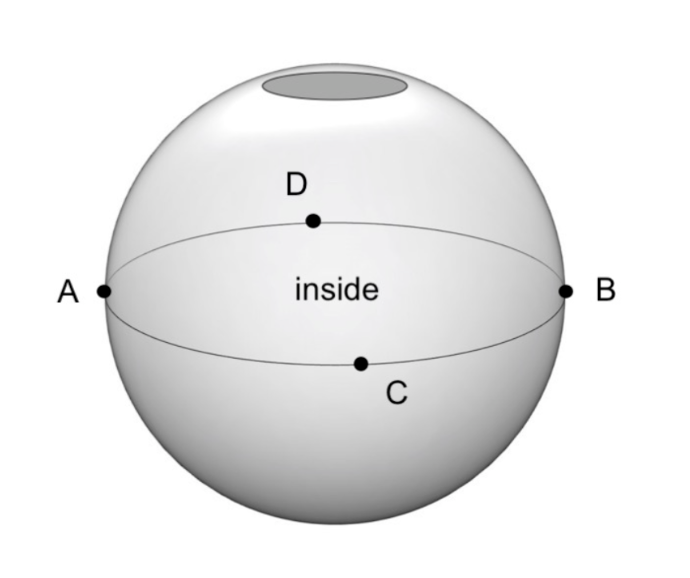
\includegraphics[height=5cm]{photos/experiment3image.png} % Adjust the height as needed
    \caption{Experiment 3: Hollow Sphere Diagram}
    \label{fig:experiment2}
\end{figure}

\begin{table}[h]
    \caption{\label{tab:table6}:  Results From The Conductive Hollow Sphere}
    \begin{tabular}{@{}rllllllll@{}}
    \toprule
    \multicolumn{1}{l}{} & \multicolumn{8}{c}{\textbf{CHARGE (V)}}                       \\ \midrule
    \multicolumn{1}{c}{\textbf{POINTS}} &
      \multicolumn{1}{c}{Trial 1} &
      \multicolumn{1}{c}{Trial 2} &
      \multicolumn{1}{c}{Trial 3} &
      \multicolumn{1}{c}{Trial 4} &
      \multicolumn{1}{c}{Trial 5} &
      \multicolumn{1}{c}{\textbf{Average}} &
      \multicolumn{1}{c}{\textbf{MR}} &
      \multicolumn{1}{c}{\textbf{ME}} \\
    A (Right - Outside)  & 4.7  & 4.2  & 4.7  & 4.8  & 4.9  & 4.66  & 0.46 & 0.205718254 \\
    B (Left - Outside)   & 5.4  & 5.3  & 6.8  & 7.8  & 6.5  & 6.36  & 1.44 & 0.643987578 \\
    C (Front - Outside)  & 5.9  & 5.5  & 5.6  & 5.3  & 5.1  & 5.48  & 0.42 & 0.18782971  \\
    D (Back - Outside)   & 6.4  & 6.7  & 6.7  & 6    & 5.2  & 6.2   & 1    & 0.447213595 \\
    Inside               & -0.1 & -0.1 & -0.2 & -0.1 & -0.4 & -0.18 & 0.22 & 0.098386991 \\ \bottomrule
    \end{tabular}
    \end{table}
    
    The results from the conductive hollow sphere, as seen in Table~\ref{tab:table6}, show a nearly uniform charge density outside the sphere. The inside of the sphere had an average charge density very close to zero (-0.18 V). Points B, C and D have similar charge densities (6.36 V, 5.48 V, 6.2 V), whereas point A has a slightly lower charge of 4.66 V.
    
    \newpage


\newpage